\documentclass[a4paper, 10pt, garamond, oneside]{book}
\usepackage{cours-preambule}

% \toggletrue{student}
% \HideSolutionstrue

\makeatletter
\renewcommand{\@chapapp}{MPSI3 -- 20 octobre 2023 -- Devoir surveillé}
\makeatother

\graphicspath{{./figures/}{./figures/E1}{./figures/E2}{./figures/P1}{./figures/P2}}

\setlist[enumerate]{resume}
\setlist[enumerate,1]{leftmargin=10pt, label=\sqenumi}
\setlist[enumerate,2]{leftmargin=20pt, label=\Alph*)}

\newcommand{\figsvg}[1]{
  \begin{center}
    \subimport{figures/}{#1}
  \end{center}
}
\newcommand{\figsvgCap}[2]{
  \begin{center}
    \subimport{figures/}{#1}
    \captionof{figure}{#2}
  \end{center}
}

\begin{document}
\setcounter{chapter}{1}
\chapter{Électrocinétique~: permanent et ordre 1\ifprof{\!\!-- corrigé}}
\label{ch:ds02}

\ifstudent{
\begin{center}
	\Large\bfseries
	\xul{Tout moyen de communication est interdit}
	\smallbreak
	\xul{Les téléphones portables doivent être éteints et rangés dans les sacs}
	\smallbreak
	\xul{Les calculatrices sont \textit{interdites}}
\end{center}
\begin{prgm}
	\vspace{6pt}
	\begin{tcb}*[cnt, bld, fontupper=\large](ror){}
		Électrocinétique, résistances et sources, circuits RC et RL
	\end{tcb}
	\vspace{-8pt}
\end{prgm}
Le devoir est composé des parties \textit{indépendantes} suivantes~:
{\Large
\begin{itemize}[label=$\diamond$]
	\bitem{Exercice 1}~: Modélisation d'un dipôle linéaire
	\bitem{Exercice 2}~: Point de fonctionnement d'une diode
	\bitem{Problème 1}~: Balise lumineuse
	\bitem{Problème 2}~: Régimes transitoires successifs d'un circuit RL
\end{itemize}
}

Les différentes questions peuvent être traitées dans l'ordre désiré.
\textbf{Cependant}, le numéro complet de la question doit être indiqué, et
\textbf{vous indiquerez si vous traitez la question d'un exercice sur une page
	complètement déconnectée}, sous peine de n'être ni vue ni corrigée.
\bigbreak
Une attention particulière sera portée à la \textbf{qualité de rédaction}. Les
hypothèses doivent être clairement énoncées, les propositions reliées entre
elles par des connecteurs logiques, les lois et théorèmes énoncés, sans pour
autant devenir une composition de français.
\bigbreak
De plus, la \textbf{présentation} de la copie sera prise en compte. Outre la
numérotation des questions, l'écriture, l'orthographe, les encadrements, la
marge, le cadre laissé pour la note et le commentaire font partie des points à
travailler. Il est notamment attendu que \textbf{les expressions littérales
	soient encadrées}, que \textbf{les calculs n'apparaissent pas} mais que le
détail des grandeurs avec leurs unités soit indiqué, et \textbf{les applications
	numériques soulignées}.
\bigbreak
Ainsi, l'étudiant-e s'expose aux malus suivants concernant la forme et le fond~:
\begin{tcb}*(prop)"bomb"{Malus}
	\begin{minipage}[t]{0.50\linewidth}
		\begin{itemize}
			\item A~: application numérique mal faite~;
			\item N~: numéro de copie manquant~;
			\item P~: prénom manquant~;
			\item E~: manque d'encadrement des réponses~;
			\item M~: marge non laissée ou trop grande~;
			\item V~: confusion ou oubli de vecteurs~;
		\end{itemize}
	\end{minipage}
	\begin{minipage}[t]{0.50\linewidth}
		\begin{itemize}
			\item Q~: question mal ou non indiquée~;
			\item C~: copie grand carreaux~;
			\item U~: mauvaise unité (flagrante)~;
			\item H~: homogénéité non respectée~;
			\item S~: chiffres significatifs non cohérents~;
			\item $\f$~: loi physique fondamentale brisée.
		\end{itemize}
	\end{minipage}
\end{tcb}

\begin{tcb}(impo){Exemple application numérique}
	\vspace*{-10pt}
	\begin{minipage}[c]{0.45\linewidth}
		\begin{gather*}
			\boxed{n = \frac{PV}{RT}}
			\qav
			\left\{
			\begin{array}{rcl}
				p & = & \SI{1.0e5}{Pa}                \\
				V & = & \SI{1.0e-3}{m^3}              \\
				R & = & \SI{8.314}{J.mol^{-1}.K^{-1}} \\
				T & = & \SI{300}{K}
			\end{array}
			\right.\\
			\mathrm{A.N.~:}\quad
			\xul{n = \SI{5.6e-4}{mol}}
		\end{gather*}
	\end{minipage}
	\hfill
	\cancel{\bcancel{
			\begin{minipage}[c]{0.45\linewidth}
				\begin{gather*}
					n = \frac{PV}{RT} = \frac{\num{e5}\cdot\num{1}}{8.32\cdot300}
					= 0.56
				\end{gather*}
			\end{minipage}
		}}
\end{tcb}
\newpage
}

\setcounter{section}{0}
\exercice[49]{Modélisation d'un dipôle linéaire}
\restartlist{enumerate}

\ifstudent{
	\noindent
	\begin{minipage}[c]{.5\linewidth}
		Dans ce problème, on étudie le dipôle AB suivant dans lequel
		le dipôle $D$ peut être un fil, un interrupteur
		ouvert ou une résistance.
	\end{minipage}
	\hfill
	\begin{minipage}[c]{.5\linewidth}
		~
		\begin{center}
			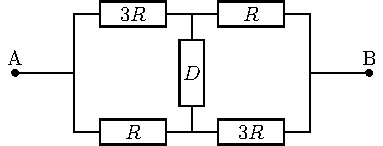
\includegraphics[scale=1]{diplin_1}
			\label{fig:diplin1}
			\captionof{figure}{}
		\end{center}
	\end{minipage}
}
\switch{
	\begin{enumerate}
		\item Exprimer la résistance $R_\infty$ du dipôle AB si $D$ est un
		      interrupteur ouvert. Faire l'application numérique.
		\item Exprimer la résistance $R_0$ du dipôle AB si $D$ est un fil.
		      Faire l'application numérique.
	\end{enumerate}
}{
	\begin{enumerate}
		\nitem{5} \label{Q:Douv}\noindent
		\begin{minipage}[t]{0.55\linewidth}
			Si $D$ est un interrupteur ouvert, alors le circuit est composé de
			deux branches parallèles, avec des résistances $R$ et $3R$ soit
			$R_{\rm serie} = R + 3R = 4R$.
			Or, pour deux résistances $R_1$ et $R_2$ en parallèle, on a
			\begin{center}
				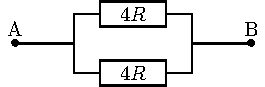
\includegraphics[width=.67\linewidth]{diplin_q1}
			\end{center}
		\end{minipage}
		\hfill
		\begin{minipage}[t]{0.4\linewidth}
			\begin{DispWithArrows*}[fleqn, mathindent=1em]
				\frac{1}{R_{\eq}} &= \frac{1}{R_1} + \frac{1}{R_2}
				\Arrow{$R_1 = R_2 = 4R$}
				\\\Lra
				\frac{1}{R_{\eq}} &= \frac{2}{4R}
				\CArrow{$\frac{1}{(~)}$}
				\\\Lra
				\Aboxed{R_{\infty}&=2R}
				\Arrow{$R = \SI{100}{\ohm}$}
				\\\Ra
				\makebox[0pt][l]{$\xul{\phantom{R_{\infty}=\SI{200}{\ohm}}}$}
				R_{\infty}&=\SI{200}{\ohm}
			\end{DispWithArrows*}
		\end{minipage}
		\nitem{4} \label{Q:Dfil}\noindent
		\begin{minipage}[t]{0.55\linewidth}
			Si $D$ est un fil, le circuit est l'association en série de deux
			résistances $R_{\eq}$ identiques correspondant à l'association en
			parallèle de la résistance $3R$ et de la résistance $R$,
			soit $R_{\eq}=3R/4$.
			\bigbreak
			\[
				\boxed{R_0 = 3R/2} \Ra \xul{R_0 = \SI{150}{\ohm}}
			\]
		\end{minipage}
		\hfill
		\begin{minipage}[t]{0.4\linewidth}
			~
			\vspace{-20pt}
			\begin{center}
				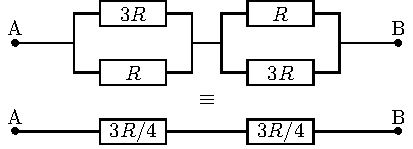
\includegraphics[width=\linewidth]{diplin_q2}
			\end{center}
		\end{minipage}
	\end{enumerate}
}
\subsection{Sur une source de tension}
\switch{
	\noindent
	\begin{minipage}[c]{.5\linewidth}
		Dans cette partie, le dipôle AB est branché sur une source de tension de
		force électromotrice constante $E$.
		Toutes les notations utilisées dans cette partie sont définies sur la
		Figure~\ref{fig:diplin2}.
	\end{minipage}
	\hfill
	\begin{minipage}[c]{.5\linewidth}
		~
		\vspace{-20pt}
		\begin{center}
			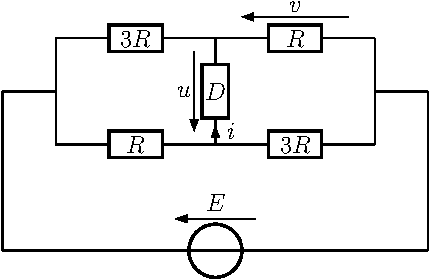
\includegraphics[scale=1]{diplin_2}
			\captionof{figure}{}
			\label{fig:diplin2}
		\end{center}
	\end{minipage}
	\begin{center}
		\bfseries
		Dans cette partie, les expressions littérales ne pourront faire intervenir
		que $E$ et $R$.
	\end{center}
	\begin{enumerate}
		\item Exprimer la tension $u$ si 	$D$ est un interrupteur ouvert.
		      Faire l'application numérique.
	\end{enumerate}
	Pour les deux questions suivantes, D est un \textbf{interrupteur fermé}.
	\begin{enumerate}
		\item Exprimer la tension $v$ dans ce cas. Faire l'application numérique.
		\item Exprimer l'intensité $i$  dans ce cas. Faire l'application numérique.
	\end{enumerate}
}{
	\begin{enumerate}
		\nitem{8} \noindent
		\begin{minipage}[t]{0.55\linewidth}
			\begin{DispWithArrows*}
				u &= U_{DC}
				\Arrow{Additivité des tensions}
				\\\Lra
				u &= U_{DB} + U_{BC}
				\Arrow{Attention au signe}
				\\\Lra
				u &= v'-v
			\end{DispWithArrows*}
			On reconnait deux ponts diviseurs de tension. Or, pour une
			résistance $R_2$ en série avec une résistance $R_1$ dans une branche
			de tension $U_{\rm brch}$, on a
			\begin{gather*}
				U_{R_k} = \frac{R_k}{R_1+R_2}U_{\rm brch}
				\\\Ra
				v'=\frac{3E}{4}
				\qet
				v=\frac{E}{4}
				\\\Ra
				\boxed{u=\frac{E}{2}}
				\Ra
				\xul{u=\SI{3}{\volt}}
			\end{gather*}
		\end{minipage}
		\hfill
		\begin{minipage}[t]{0.4\linewidth}
			~
			\vspace{-40pt}
			\begin{center}
				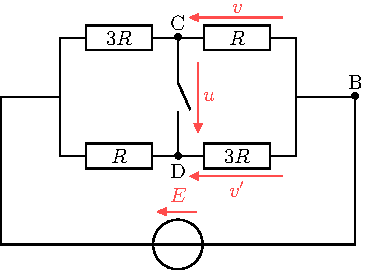
\includegraphics[width=\linewidth]{diplin_q3}
			\end{center}
		\end{minipage}
		\nitem{3}
		\noindent
		\begin{minipage}[t]{0.55\linewidth}
			Dans ce cas, d'après la question~\ref{Q:Dfil}, la tension $v$
			correspond à la tension aux bornes de la résistance équivalente
			$R_{\eq} = 3R/4$.

			On applique la formule du pont diviseur de tension sur l'association
			en série des deux résistances $R_{\eq}$~:
			\[
				\boxed{v = E/2}
				\Ra
				\xul{v=\SI{3}{\volt}}
			\]
		\end{minipage}
		\hfill
		\begin{minipage}[t]{0.4\linewidth}
			~
			\vspace{-30pt}
			\begin{center}
				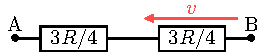
\includegraphics[width=\linewidth]{diplin_q4}
			\end{center}
		\end{minipage}
		\vspace{30pt}
		\nitem{5} \noindent
		\begin{minipage}[t]{0.55\linewidth}
			Par l'application de la loi des nœuds et de la loi d'Ohm~:
			\begin{gather*}
				i=i_2-i_1=\frac{v}{R}-\frac{v}{3R}
				\\\Lra
				\boxed{i = \frac{E}{3R}}
				\Ra
				\xul{i = \SI{20}{\milli\ampere}}
			\end{gather*}
		\end{minipage}
		\hfill
		\begin{minipage}[t]{0.4\linewidth}
			~
			\vspace{-60pt}
			\begin{center}
				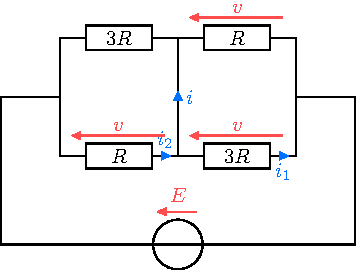
\includegraphics[width=\linewidth]{diplin_q5}
			\end{center}
		\end{minipage}
	\end{enumerate}
}
\subsection{Sur une source de courant}
\switch{
	\noindent
	\begin{minipage}[c]{.5\linewidth}
		Dans cette partie, le dipôle AB est branché sur une source de courant, dont
		le courant électromoteur $I_0$ est constant. Toutes les notations utilisées
		dans cette partie sont définies sur la Figure~\ref{fig:diplin3}
	\end{minipage}
	\hfill
	\begin{minipage}[c]{.5\linewidth}
		~
		\vspace{-20pt}
		\begin{center}
			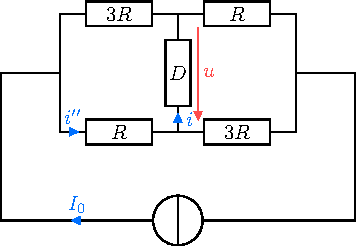
\includegraphics[scale=1]{diplin_3}
			\captionof{figure}{}
			\label{fig:diplin3}
		\end{center}
	\end{minipage}
	\begin{center}
		\bfseries
		Dans cette partie, les expressions littérales ne pourront faire intervenir
		que $I_0$ et $R$.
	\end{center}
	\begin{enumerate}
		\item Exprimer la tension $u$ si 	$D$ est un interrupteur ouvert.
		      Faire l'application numérique.
	\end{enumerate}
	Pour les deux questions suivantes, D est un \textbf{interrupteur fermé}.
	\begin{enumerate}
		\item Exprimer l'intensité $i''$. Faire l'application numérique.
		\item Exprimer l'intensité $i$ dans ce cas. Faire l'application numérique.
	\end{enumerate}
}{
	\begin{enumerate}
		\nitem{5} \noindent
		\begin{minipage}[t]{0.55\linewidth}
			Si $D$ est un interrupteur ouvert, alors le courant est le même
			dans les deux branches qui ont la même résistance équivalente,
			donc $i''=I_0/2$ avec la loi des nœuds.
			\smallbreak
			Or, par l'additivité des tensions, $u=u'-u''$. En appliquant la loi
			d'Ohm, on obtient
			\[
				\boxed{u = RI_0}
				\Ra
				\xul{u = \SI{4}{\volt}}
			\]
		\end{minipage}
		\hfill
		\begin{minipage}[t]{0.4\linewidth}
			~
			\vspace{-40pt}
			\begin{center}
				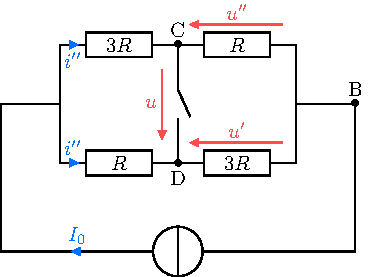
\includegraphics[width=\linewidth]{diplin_q6}
			\end{center}
		\end{minipage}
		\nitem{4} \noindent
		\begin{minipage}[t]{0.55\linewidth}
			On reconnaît les conditions d'application d'un pont diviseur de
			courant~: pour deux résistances $R_1$ et $R_2$ en parallèle
			alimentées par un courant $I_0$ se divisant en $i_1$ et $i_2$
			respectivement, on a
			\begin{gather*}
				i'' = \frac{G_1}{G_1+G_2}I_0
				\Ra
				i'' = \frac{\frac{1}{R}}{\frac{1}{R}+\frac{1}{3R}}I_0
				\Lra
				i'' = \frac{\frac{1}{R}}{\frac{4}{3R}}I_0
				\\\Lra
				\boxed{i'' = \frac{3}{4}I_0}
				\Ra
				\xul{i'' = \SI{30}{mA}}
			\end{gather*}
		\end{minipage}
		\hfill
		\begin{minipage}[t]{0.4\linewidth}
			~
			\vspace{-20pt}
			\begin{center}
				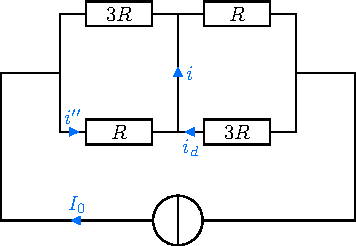
\includegraphics[width=\linewidth]{diplin_q8}
			\end{center}
		\end{minipage}
		\nitem{4} D'après la formule du pont diviseur de courant, $i_d=-I_0/4$.
		Ainsi,
		\[
			i = i'' + i_d
			\Lra
			\boxed{i = \frac{I_0}{2}}
			\Ra
			\xul{i = \SI{20}{mA}}
		\]
	\end{enumerate}
}
\subsection{Application}
\switch{
	\noindent
	\begin{minipage}[c]{.5\linewidth}
		On admet qu'il existe quatre constantes $a$, $b$, $c$ et $d$ telles que
		\begin{align*}
			u' & =a i + b u \\
			i' & = c i + du
		\end{align*}
		quels que soient les dipôles $D$ et $D'$ dans le circuit
		Figure~\ref{fig:diplin4}.
	\end{minipage}
	\hfill
	\begin{minipage}[c]{.5\linewidth}
		~
		\vspace{-20pt}
		\begin{center}
			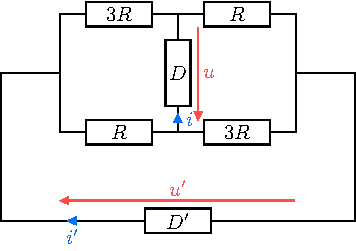
\includegraphics[scale=1]{diplin_4}
			\captionof{figure}{}
			\label{fig:diplin4}
		\end{center}
	\end{minipage}
	\begin{enumerate}
		\item Exprimer les constantes $a$, $b$, $c$ et $d$.
	\end{enumerate}
	Pour les trois questions suivantes, D est une résistance $\rho$.
	\begin{enumerate}
		\item Exprimer la résistance équivalente $R_{AB}$ du dipôle AB en
		      fonction des résistances $R$ et $\rho$.
		\item Que devient l'expression précédente dans la limite $\rho \ra \infty$~?
		      Commenter.
		\item Que devient l'expression précédente dans la limite $\rho \ra 0$~?
		      Commenter.
	\end{enumerate}
}{
	\begin{enumerate}
		\nitem{4} Dans le cas où $D'$ est un générateur de tension de f.e.m. $u'=E$~:
		\begin{itemize}
			\item Si $D$ est un interrupteur ouvert, $i=0$ et $u=E/2$~:
			      $E=bE/2$, donc $\boxed{b=2}$
			\item Si $D$ est un fil, $u=0$ et $i=E/(3R)$~: $E=aE/(3R)$, donc
			      $\boxed{a=3R}$
		\end{itemize}
		Dans le cas où $D'$ est un générateur de courant de c.e.m. $i'=I_0$~:
		\begin{itemize}
			\item Si $D$ est un fil, $u=0$ et $i=I_0/2$~: $I_0=cI_0/2$,
			      donc $\boxed{c=2}$
			\item Si $D$ est un interrupteur ouvert, $i=0$ et $u=RI_0$~:
			      $I_0=dRI_0$, donc $\boxed{d=1/R}$
		\end{itemize}
		\nitem{3} Par application de la loi d'Ohm sur le dipôle AB, et sur la
		résistance
		$\rho$~:
		\[
			R_{AB}=u'/i'
			\qet
			u=\rho i
		\]
		On remplace $u$ dans les expressions de $u'$ et de $i'$ :
		\[
			u'=(3R+2\rho)i
			\qet
			i'=\left (2+\frac{\rho}{R}\right )i
		\]
		En faisant le rapport des deux, on obtient la résistance équivalente :
		\[
			\boxed{R_{AB}=R\times \frac{3R+2\rho}{2R+\rho}}
		\]
		\nitem{2} $\lim_{\rho\rightarrow \infty }R_{AB}=2R=R_\infty$, il y a cohérence
		avec la réponse à la question~\ref{Q:Douv}.
		\nitem{2} $\lim_{\rho\rightarrow 0}R_{AB}=3R/2=R_0$, il y a cohérence avec la
		réponse à la question~\ref{Q:Dfil}.
	\end{enumerate}
}

\newpage

\exercice[39]{Point de fonctionnement d'une diode}
\restartlist{enumerate}

\switch{
	On considère une diode en silicium dont la caractéristique courant/tension est
	représentée sur la figure~\ref{fig:carac_diode}. La diode est dite bloquée
	quand la tension à ses bornes $u_D$ est inférieure à sa tension seuil $u_s$.
	La diode est dite passante dans le cas contraire.

	On prendra $u_s=\SI{0,60}{\volt}$. On donne les coordonnées du point $C$~:
	$i_C=\SI{500}{\milli\ampere}$ et $u_C=\SI{0,70}{\volt}$.

	\noindent
	\begin{minipage}[t]{.5\linewidth}
		\begin{center}
			\subimport{figures/E2/}{diode_carac.pdf_tex}
			\captionof{figure}{Caractéristique d'une diode silicium.}
			\label{fig:carac_diode}
		\end{center}
	\end{minipage}
	\begin{minipage}[t]{.5\linewidth}
		\begin{center}
			\subimport{figures/E2/}{diode_thevenin.pdf_tex}
			\captionof{figure}{Modèle de \textsc{Thévenin}}
			\label{fig:thevenin}
		\end{center}
	\end{minipage}
	\begin{enumerate}
		\item Dans le cas où la diode est bloquée, par quel dipôle peut-on la
		      modéliser~?
		\item Dans le cas où la diode est passante, le courant vérifie
		      $i_D=a\cdot u_D+b$. Exprimer $a$ et $b$ en fonction de $u_s$, $i_C$
		      et $u_C$. Calculer $a$ et $b$.
	\end{enumerate}

	On veut montrer que la diode peut être modélisée par un générateur de
	Thévenin de f.e.m. $e$ et de résistance $r$ (figure~\ref{fig:thevenin})
	lorsqu'elle est passante.
	\begin{enumerate}
		\item Exprimer $i$ en fonction de $u$, $e$ et $r$.
		\item En déduire les expressions de $e$ et $r$ en fonction de $a$ et $b$
		      pour que la diode soit équivalente au générateur de Thévenin lorsqu'elle
		      est passante. Calculer $e$ et $r$.
	\end{enumerate}
	On considère le circuit de la figure~\ref{fig:circuit_diode1} constitué de la
	diode précédente, d'un générateur de tension idéal de f.e.m. $e_1$ et de deux
	résistances identiques $R$.
	\smallbreak
	\noindent
	\begin{minipage}[t]{.5\linewidth}
		\begin{center}
			\subimport{figures/E2/}{diode_1.pdf_tex}
			\captionof{figure}{Circuit électrique étudié.}
			\label{fig:circuit_diode1}
		\end{center}
	\end{minipage}
	\begin{minipage}[t]{.5\linewidth}
		\begin{center}
			\subimport{figures/E2/}{diode_2.pdf_tex}
			\captionof{figure}{Étude du dipôle générateur.}
			\label{fig:circuit_diode2}
		\end{center}
	\end{minipage}
	\begin{enumerate}
		\item On suppose que la diode est bloquée. Refaire le circuit électrique.
		      En déduire l'inégalité vérifiée par $e_1$ pour que cette hypothèse soit
		      vérifiée.
		\item On suppose que la diode est passante. Refaire le circuit. Exprimer
		      $u_D$ en fonction de $e_1$, $e$, $R$ et $r$. Calculer $u_D$ avec
		      $e_1=\SI{10}{\volt}$ et $R=\SI{4.0}{\ohm}$. En déduire la valeur de $i_D$.
	\end{enumerate}

	On souhaite retrouver ce résultat graphiquement en utilisant le point de
	fonctionnement.
	\begin{enumerate}
		\item Exprimer $i'$ en fonction de $u'$ pour le circuit représenté sur la
		      figure~\ref{fig:circuit_diode2}.
		\item Tracer la solution trouvée sur la Figure~\ref{fig:diode_annexe} en
		      annexe. En déduire graphiquement les coordonnées du point de
		      fonctionnement. Conclure.
	\end{enumerate}
}
{
	\begin{enumerate}
		\nitem{2} Une diode bloquée est modélisable par un interrupteur ouvert
		($i=0$).
		\nitem{5} Le coefficient directeur est donné par le taux d'accroissement
		\[
			\boxed{a=\frac{i_C}{u_C-u_s}}
			\qav
			\left\{
			\begin{array}{rcl}
				i_C & = & \SI{0.500}{A}
				\\
				u_C & = & \SI{0.70}{V}
				\\
				u_s & = & \SI{0.60}{V}
			\end{array}
			\right.
			\quad \Ra \quad
			\xul{
				a=\SI{5.0}{\siemens}
			}
		\]
		Pour déterminer l'ordonnée à l'origine, on utilise le point
		d'abscisse $u_s$ et d'ordonnée nulle~:
		\[
			0=au_s+b\qso
			\boxed{b=-au_s=\frac{-i_Cu_s}{u_C-u_s}}
			\Ra
			\xul{b=\SI{-3.0}{\ampere}}
		\]
		\nitem{2} D'après l'additivité des tensions et la loi d'Ohm, $u=ri-e$, soit
		$\boxed{i = \frac{e}{r} + \frac{u}{r}}$.
		\nitem{6} Deux dipôles sont équivalents s'ils ont la même caractéristique. On
		en déduit $i=i_D$ si $u=u_D$, soit $e/r=b$ et $1/r=a$~:
		\[
			\boxed{r=1/a=\SI{0,20}{\ohm}}
			\qet
			\boxed{e=b/a=-u_s=\SI{-0,60}{\volt}}
		\]
		\nitem{5}
		\noindent
		\begin{minipage}[t]{.55\linewidth}
			En remplaçant la diode par un interrupteur, on reconnait un pont
			diviseur de tension~: $u_D=\frac{e_1}{2}$. La diode est bloquée si
			$u_D<u_s$, donc il faut que
			\[
				\boxed{e_1<2u_s}
			\]
		\end{minipage}
		\hfill
		\begin{minipage}[t]{.4\linewidth}
			~
			\vspace{-40pt}
			\begin{center}
				\subimport{figures/E2/}{diode_corr3.pdf_tex}
			\end{center}
		\end{minipage}
		\nitem{10}
		\noindent
		\begin{minipage}[t]{.55\linewidth}
			On refait le circuit en faisant attention à l'orientation de la
			tension $e$.
			La loi des nœuds et les lois d'Ohm sont appliquées sur le schéma.
			On définit $u_D$ comme étant la tension aux bornes des trois
			branches en parallèle~:
			\begin{align}
				u_D & =e_1-Ri_1\label{eq:uD1}
				\\\Lra
				u_D & =R(i_1-i_D)\label{eq:uD2}
				\\\Lra
				u_D & =ri_D-e\label{eq:uD3}
			\end{align}
		\end{minipage}
		\hfill
		\begin{minipage}[t]{.4\linewidth}
			~
			\vspace{-30pt}
			\begin{center}
				\subimport{figures/E2/}{diode_corr.pdf_tex}
			\end{center}
		\end{minipage}

		\begin{gather*}
			\eqref{eq:uD1}+\eqref{eq:uD2}\Ra
			2u_D=e_1-Ri_D
			\qso
			i_D=\frac{e_1-2u_D}{R}
			\\
			\eqref{eq:uD3}\Ra
			u_D=\frac{r}{R}(e_1-2u_D)-e
			\qso
			\boxed{u_D=\frac{re_1-Re}{2r+R}}
			\qav
			\left\{
			\begin{array}{rcl}
				r   & = & \SI{0.20}{\ohm}
				\\
				e_1 & = & \SI{10}{V}
				\\
				R   & = & \SI{4.0}{\ohm}
				\\
				e   & = & \SI{-0.60}{V}
			\end{array}
			\right.\\
			\AN
			\xul{
				u_D=\SI{1.0}{\volt}
			}
		\end{gather*}
		On remarque que $u_D>u_s$, donc la \xul{diode est bien passante}.
		Pour trouver $i_D$ on utilise la caractéristique de la diode~:
		\[
			\boxed{i_D=au_D+b} \Ra \xul{i_D=\SI{2.0}{\ampere}}
		\]
		\nitem{5} \noindent
		\begin{minipage}[t]{.55\linewidth}
			Loi des mailles et loi d'Ohm~:
			\begin{DispWithArrows*}
				u' = e_1-Ri_1
				\quad & \text{et} \quad
				u' = Ri_2
				\Arrow{On isole}
				\\\Lra
				i_1 = \frac{e_1-u'}{R}
				\quad & \text{et} \quad
				i_2 = u'/R
				\Arrow{$i' = i_1 - i_2$}
				\\\Ra
				\Aboxed{i' = \frac{e_1}{R}&-\frac{2}{R}u'}
			\end{DispWithArrows*}
		\end{minipage}
		\hfill
		\begin{minipage}[t]{.4\linewidth}
			~
			\vspace{-30pt}
			\begin{center}
				\subimport{figures/E2/}{diode_corr2.pdf_tex}
			\end{center}
		\end{minipage}
		\nitem{4} Voir Figure~\ref{fig:diode_annexecorr}. On lit les coordonnées du
		point d'intersection $I(\SI{1.0}{\volt};\SI{2.0}{\ampere})$. Cela
		correspond aux valeurs déterminées précédemment.
	\end{enumerate}
}

\newpage

\setcounter{section}{0}
\prblm[45]{Balise lumineuse}
\restartlist{enumerate}
\switch{
	\noindent
	\begin{minipage}[t]{.5\linewidth}
		~
		\begin{center}
			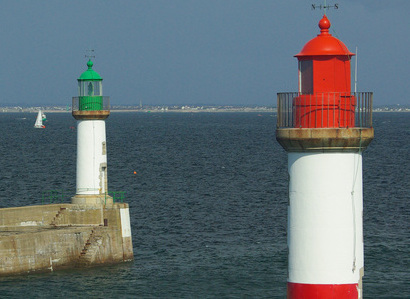
\includegraphics[width=.65\linewidth]{balise_photo}
			\captionof{figure}{Photo d'une balise lumineuse.}
		\end{center}
	\end{minipage}
	\hfill
	\begin{minipage}[t]{.5\linewidth}
		~
		\begin{center}
			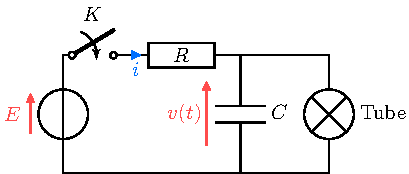
\includegraphics[width=\linewidth]{balise_schema_main}
			\captionof{figure}{Schéma électrique associé.}
		\end{center}
	\end{minipage}
	\smallbreak
	La passe des ports est signalée la nuit par une balise lumineuse dont le
	schéma électrique est donné ci-dessus.
	La source de lumière est constituée d'un tube à décharge. La décharge
	électrique qui se produit entre les électrodes du tube est caractérisée par
	une tension d'allumage $U_{a}$ et une tension d'extinction $U_{ex}$. On a~:
	\begin{itemize}
		\item Le tube s'allume lorsque la tension à ses bornes prend une valeur qui
		      devient supérieure à $U_{a}$, il se comporte alors comme un résistor de
		      résistance $r \ll R$.
		\item Il s'éteint lorsque la tension à ses bornes prend une valeur qui
		      devient inférieure à $U_{ex}$, il se comporte alors comme un résistor de
		      résistance supposée infinie.
		\item Il s'allume à nouveau lorsque la tension à ses bornes redevient
		      supérieure à $U_{a}$.
	\end{itemize}
	On suppose que $E > U_{a}  > U_{ex}$ et on pose $\tau = RC$ ainsi que
	$\tau' = rC$. À l'instant initial $t = 0$, le condensateur n'est pas chargé
	et on ferme l'interrupteur $K$.
	\bigbreak
	Ainsi, lors de la charge du condensateur de constante de temps $\tau$,
	le tube est éteint (sa résistance est infinie), et lors de la décharge
	très rapide de constante de temps $\tau'$ à travers le tube (sa
	résistance est alors $r$), le tube est allumé.
	\begin{enumerate}
		\item Déterminer le comportement du tube à l'instant initial.
		      En déduire le schéma équivalent du circuit et l'équation
		      différentielle vérifiée par $v(t)$, puis la résoudre.
		\item Déterminer l'expression de l'instant $t_{a}$ où s'amorce la décharge
		      (allumage du tube).
		\item On se place maintenant dans le régime où la lampe est allumée.
		      Le circuit électrique est alors modifié et il convient de déterminer
		      la nouvelle équation différentielle. Montrer que l'équation
		      différentielle à laquelle satisfait $v(t)$ à partir de cet instant
		      s'écrit avant simplification~:
		      \[
			      E = RC \dv{v}{t} + \left(\frac{R}{r}+1\right) v
		      \]
		      \noindent
		      On utilisera la condition $r \ll R$ pour simplifier l'expression. On
		      supposera également que $v(t) \gg (r/R)E$ durant cette phase. Montrer
		      que l'expression précédente devient alors
		      \[
			      0 = rC \dv{v}{t} + v
		      \]
		      \noindent
		      En déduire alors l'expression de $v(t)$.
		\item Déterminer l'expression de l'instant $t_{ex}$ où se produit
		      l'extinction du tube.
		\item En déduire l'expression de la durée $T_1$ de l'éclair produit dans le
		      tube.
		\item Déterminer l'expression du temps $T_2$ qui s'écoule entre l'extinction
		      et l'allumage suivant en fonction de $\tau$, $E$, $U_{ex}$  et $U_{a}$.
		\item En déduire l'expression de la période $T$ des éclairs produits par ce
		      dispositif.
		\item Numériquement, on obtient
		      \[
			      T_1 = \SI{2,5e-7}{\second}
			      \quad , \quad
			      T_2 = \SI{1,0}{\second}
			      \qet
			      T = \SI{1,0}{\second}
		      \]
		      Que peut-on en conclure~?
	\end{enumerate}
}{
	\begin{enumerate}
		\nitem{16}
		\noindent
		\begin{minipage}[t]{.55\linewidth}
			La tension aux bornes d'un condensateur est une fonction continue du
			temps donc $v(t=0^+)=v(t=0^-)=0<U_{a}$. Le tube est par conséquent
			éteint et la lampe est donc assimilable à un interrupteur ouvert.
			Avec une loi des mailles~:
			\begin{DispWithArrows*}[]
				u_R(t) + v(t) &= E
				\Arrow{$u_R(t) = Ri(t)$}
				\\\Lra
				Ri(t) + v(t) &= E
				\Arrow{$i(t) = C \dv{v}{t}$}
				\\\Lra
				RC \dv{v}{t} + v(t) &= E
				\Arrow{$\tau = RC$}
				\\\Lra
				\Aboxed{\dv{v}{t} + \frac{v(t)}{\tau} &= \frac{E}{\tau}}
			\end{DispWithArrows*}
		\end{minipage}
		\hfill
		\begin{minipage}[t]{.4\linewidth}
			~
			\vspace{-25pt}
			\begin{center}
				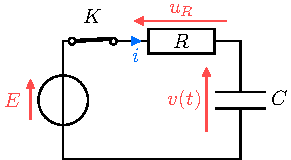
\includegraphics[width=\linewidth]{balise_q1}
			\end{center}
		\end{minipage}
		\begin{isd}[lefthand ratio=.4]
			L'équation homogène est
			\[
				\dv{v_h}{t} + \frac{v_h}{\tau} = 0
			\]
			de solution
			\[
				v_h(t) = A\exr^{-t/\tau}
			\]
			Une solution particulière $v_p(t) = \lambda$ donne
			\[
				\underbracket[1pt]{\cancel{\dv{\lambda}{t}}}_{=0} +
				\frac{\lambda}{\tau} = E
				\Lra
				\boxed{\lambda = E}
			\]
			\tcblower
			\begin{DispWithArrows*}[]
				v(t) &= v_h(t) + v_p
				\Arrow{On remplace}
				\\\Lra
				v(t) &= A\exr^{-t/\tau} + E
				\Arrow{Condition initiale}
				\\
				\text{or,} \quad
				v(0) &= A+E = 0
				\Arrow{On isole $A$}
				\\\Lra
				\Aboxed{A &= -E}
				\Arrow{On combine}
				\\\Ra
				\Aboxed{v(t) &= E \left( 1-\exr^{-t/\tau} \right)}
			\end{DispWithArrows*}
		\end{isd}
		\nitem{3} La décharge s'amorce à l'instant $t_{a}$ tel que $v(t_{a}) =
			U_{a}$. Soit
		\begin{DispWithArrows*}
			E\left(1-\exr^{-t_{a}/\tau}\right) &= U_{a}
			\CArrow{$\mdiv E$}
			\\\Lra
			1 - \exr^{-t_a/\tau} &= \frac{U_a}{E}
			\Arrow{On isole $\exr^{-t_a/\tau}$}
			\\\Lra
			\exr^{-t_a/\tau} &= \frac{E-U_a}{E}
			\CArrow{$\ln(~)$}
			\\\Lra
			\frac{-t_a}{\tau} &= \ln (\frac{E-U_a}{E})
			\Arrow{$-\ln (a) = \ln (\frac{1}{a})$}
			\\\Lra
			\Aboxed{t_a &= \tau \ln (\frac{E}{E-U_a})}
		\end{DispWithArrows*}
		\nitem{11}
		\noindent
		\begin{minipage}[t]{.4\linewidth}
			La lampe est maintenant assimilable à une résistance $r$. On obtient
			alors le nouveau schéma équivalent~:
			\begin{center}
				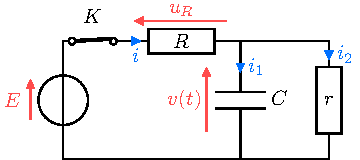
\includegraphics[width=\linewidth]{balise_q3}
			\end{center}
		\end{minipage}
		\hfill
		\begin{minipage}[t]{.55\linewidth}
			Avec une loi des mailles et la loi d'Ohm~:
			\begin{DispWithArrows*}[fleqn, mathindent=5pt]
				u_R + v &= E
				\Arrow{Loi d'Ohm}
				\\\Lra
				Ri + v &= E
				\Arrow{$i = i_1+i_2$}
				\\\Lra
				R(i_1 + i_2) + v &= E
				\Arrow{$i_1 = C \dv{v}{t}$\\et $i_2 = \frac{v}{r}$}
				\\\Lra
				R \left( C \dv{v}{t} + \frac{v}{r} \right) + v &= E
				\Arrow[jump=2]{On simplifie}
				\\\Lra
				RC \dv{v}{t} + \left(\frac{R}{r}+1\right) v &= E
				\\\Lra
				rC\dv{v}{t}+ \left(1+\frac{r}{R}\right)v &= \frac{r}{R}E
				\Arrow{On néglige les termes en $\frac{r}{R}$}
				\\\Ra
				\Aboxed{rC \dv{v}{t} + v &= 0}
				\Arrow{$\tau' = rC$}
				\\
				\dv{v}{t} + \frac{v}{\tau'} &= 0
			\end{DispWithArrows*}
		\end{minipage}
		Ainsi,
		\begin{DispWithArrows*}[]
			v(t) &= A'\exr^{-t/\tau'}
			\Arrow{Condition initiale}
			\\
			\text{or,} \quad
			v(t_a) &= A'\exr^{-t_a/\tau'} = U_a
			\Arrow{On isole $A'$}
			\\\Lra
			\Aboxed{A' &= U_a\exr^{t_a/\tau'}}
			\Arrow{On combine}
			\\\Ra
			\Aboxed{v(t) &= Ua \exr^{-(t-t_a)/\tau'}}
		\end{DispWithArrows*}
		\nitem{3} La décharge se termine à l'instant $t_{ex}$ tel que
		$v(t_{ex}) = U_{ex}$. Soit
		\begin{DispWithArrows*}
			U_{a} \exr^{-(t_{ex}-t_{a})/\tau'} &= U_{ex}
			\CArrow{$\mdiv U_a$}
			\\\Lra
			\exr^{-(t_{ex}-t_{a})/\tau'} &= \frac{U_{ex}}{U_a}
			\CArrow{$\ln(~)$}
			\\\Lra
			-\frac{t_{ex} - t_a}{\tau'} &= \ln (\frac{U_{ex}}{U_a})
			\Arrow{$-\ln (a) = \ln (\frac{1}{a})$}
			\\\Lra
			\Aboxed{t_{ex} &= t_{a}+ \tau' \ln\pa{\frac{U_{a}}{U_{ex}}}}
		\end{DispWithArrows*}
		\mitem{2}
		\[
			% \vspace{-12pt}
			\boxed{
			T_1 =
			t_{ex}-t_{a} =
			\tau' \ln\pa{\frac{U_{a}}{U_{ex}}}}
		\]
		\nitem{6} Par analogie directe avec la première question, dans cette phase,
		\[
			v(t) = A'' \exr^{-t/\tau} +E \qet \tau = RC
		\]
		\noindent
		La nouvelle condition initiale s'écrit désormais
		$v(t=t_{ex}) = U_{ex}$. Soit
		\[
			A'' \exr^{-t_{ex}/\tau} + E = U_{ex}
			\quad \Lra \quad
			A'' = (U_{ex}-E) \exr^{t_{ex}/\tau}
		\]
		\leftcenters{Dont on déduit, après calcul,}
		{$\boxed{v(t) = (U_{ex}-E)\exr^{-(t-t_{ex})/\tau} + E}$}.
		\smallbreak
		Le nouvel allumage de la lampe est réalisée à la condition
		$v(t = t_{ex} + T_2) = U_{a}$, soit
		\begin{gather*}
			(U_{ex}-E)\exr^{-T_2/\tau} + E = U_{a}
			\\
			\text{D'où}\qquad
			\boxed{T_2 = \tau \ln\pa{\frac{U_{ex}-E}{U_{a}-E}}}
		\end{gather*}

		\mitem{2} \[
			T = T_1+T_2
			\Lra
			\boxed{
				T =
				\tau \ln\left(\frac{U_{ex}-E}{U_{a}-E}\right) +
				\tau' \ln(\frac{U_{a}}{U_{ex}})}
		\]
		\nitem{2}
		Les flashs lumineux sont très brefs devant la durée entre deux flashs,
		permettant de bien les distinguer d'un autre signal lumineux (phare).
	\end{enumerate}
}

\newpage

\prblm[84]{Régimes transitoires successifs d'un circuit RL}
\restartlist{enumerate}

\ifstudent{
\noindent
\begin{minipage}[c]{.6\linewidth}
	Le circuit ci-contre, alimenté par un générateur de tension continue $E$,
	est constitué d'une bobine d'inductance $L=\SI{100}{\milli\henry}$, de
	trois résistors de même résistance $R=\SI{100}{\ohm}$ et de deux
	interrupteurs $K_1$ et $K_2$.
	\begin{itemize}
		\item Les deux interrupteurs sont ouverts depuis longtemps quand à
		      $t=0$ on ferme l'interrupteur $K_1$ (l'interrupteur $K_2$ reste
		      ouvert).
		\item À l'instant $t_1=\SI{5.0}{\milli\second}$, on ferme $K_2$
		      (l'interrupteur $K_1$ est toujours fermé).
		\item Enfin à l'instant $t_2=\SI{10}{\milli\second}$, on ouvre $K_1$
		      ($K_2$ reste fermé).
	\end{itemize}
\end{minipage}
\hfill
\begin{minipage}[c]{.4\linewidth}
	~
	\begin{center}
		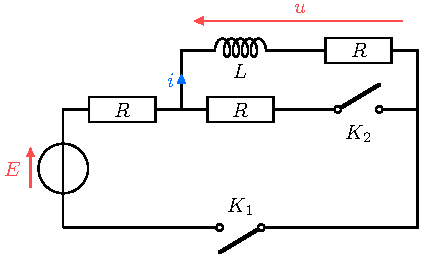
\includegraphics[scale=1]{transRL_main}
		\captionof{figure}{Schéma général.}
		\label{fig:transRL_main}
	\end{center}
\end{minipage}
Le but de l'exercice est d'étudier $i(t)$ et $u(t)$ pour $t\in]0,+\infty[$.
Pour cela, l'exercice est décomposé en \textbf{parties indépendantes}.
Seules les deux dernières questions nécessitent d'avoir traité l'ensemble
de l'exercice.
}
\subsection{Étude pour $t\in]0,t_1[$}
\switch{
	\begin{enumerate}
		\item \label{Q:CI1}
		      Exprimer l'intensité $i$ et la tension $u$ à l'instant $t=0^+$,
		      juste après la fermeture de l'interrupteur~$K_1$. Un schéma est
		      attendu.
		\item \label{Q:perm1}
		      En supposant que le régime permanent est atteint à l'instant
		      $t=t_1^-$, exprimer $i(t_1^-)$ et $u(t_1^-)$. Un schéma est attendu.
		\item Établir l'équation différentielle vérifiée par $i(t)$ pour
		      $t\in]0,t_1[$. Montrer qu'elle peut se mettre sous la forme~:
		      \[
			      \dv{i}{t}+\frac{1}{\tau_1}i=A_1
		      \]
		      Exprimer les constantes $\tau_1$ et $A_1$ en fonction des données du
		      problème.
		\item Résoudre cette équation différentielle. On exprimera $i$ en fonction
		      de $E$, $R$, $\tau_1$ et $t$ pour $t\in]0,t_1[$. Vérifier que cette
		      solution est en accord avec la réponse à la question~\ref{Q:perm1}.
		\item Exprimer $u(t)$ pour $t\in]0,t_1[$. Vérifier que cette solution est
		      en accord avec les réponses aux questions~\ref{Q:CI1} et~\ref{Q:perm1}.
		\item On enregistre les grandeurs $u$ et $i$ au cours du temps à partir de
		      $t=0$. Les graphiques sont donnés en annexe,
		      Figure~\ref{fig:annexe_p2-1}. Placer sur ces deux
		      graphiques le temps $\tau_1$. Déterminer les valeurs de $E$, $R$ et
		      $L$. Peut-on considérer que le circuit est en régime permanent à
		      l'instant $t=t_1^-$~?
	\end{enumerate}
}{
	\begin{enumerate}
		\nitem{6} \label{Q:CI1}\noindent
		\begin{minipage}[t]{.49\linewidth}
			À l'instant $t=0^-$, le circuit est en régime permanent, et les
			interrupteurs sont ouverts. Comme le circuit est ouvert, il n'y a
			pas de courant circulant dans le circuit.
			Par continuité de l'intensité traversant la bobine, on en déduit
			$\boxed{i(0^+)=i(0^-)=0}$.
			Comme il n'y a pas de courant à $t=0^+$, les tensions aux bornes des
			résistances sont nulles. En appliquant la loi des mailles~:
			$\boxed{u(0^+)=E}$
		\end{minipage}
		\hfill
		\begin{minipage}[t]{.49\linewidth}
			~
			\vspace{-20pt}
			\begin{center}
				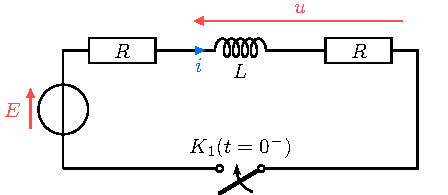
\includegraphics[width=\linewidth]{transRL_q1}
				\captionof{figure}{Schéma à $t=0^{-}$.}
			\end{center}
		\end{minipage}
		\vspace{10pt}
		\nitem{4} \label{Q:perm1}\noindent
		\begin{minipage}[t]{.49\linewidth}
			En régime permanent, la bobine se comporte comme un fil. Le
			circuit se résume à un générateur alimentant deux résistances~:
			\[
				\boxed{
					i(t_1^-)=\frac{E}{2R}
					\qet
					u(t_1^-)=\frac{E}{2}
				}
			\]
		\end{minipage}
		\hfill
		\begin{minipage}[t]{.49\linewidth}
			~
			\vspace{-30pt}
			\begin{center}
				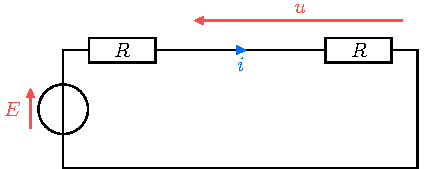
\includegraphics[width=\linewidth]{transRL_q2}
				\captionof{figure}{Schéma à $t=t_1^{-}$.}
			\end{center}
		\end{minipage}
		\nitem{5} On utilise le circuit en régime transitoire pour $t\in]0,t_1[$. On
		applique la loi des mailles~:
		\begin{gather*}
			E=Ri+L\dv{i}{t}+Ri
			\qso
			\dv{i}{t}+\frac{2R}{L}i=\frac{E}{L}
			\\
			\Ra
			\boxed{\tau_1=\frac{L}{2R}\qet A_1=\frac{E}{L}}
		\end{gather*}
		\nitem{8} On a~:
		\smallbreak
		\begin{isd}[lefthand ratio=.4]
			Équation homogène~:
			\[
				\dv{i_h}{t} + \frac{i_h}{\tau_1} = 0
			\]
			de solution
			\[
				i_h = B_1\exr^{-t/\tau_1}
			\]
			Une solution particulière $i_p (t) = \lambda$ donne
			\[
				\underbracket{\cancel{\dv{\lambda}{t}}}_{=0} +
				\frac{\lambda}{\tau_1} = \frac{E}{L}
				\Lra
				\boxed{\lambda = \frac{E}{2R}}
			\]
			\tcblower
			\begin{DispWithArrows*}[fleqn, mathindent=5pt, groups]
				i(t) &= i_h(t)+i_p(t)
				\Arrow{On remplace}
				\\\Lra
				i(t) &= B_1\exp(-t/\tau_1)+\frac{E}{2R}
				\Arrow{Condition initiale}
				\\
				\text{or,} \quad
				i(0) &= 0 = B_1+\frac{E}{2R}
				\Arrow{On isole $B_1$}
				\\\Lra
				\Aboxed{B_1 &= -\frac{E}{2R}}
				\Arrow[new-group]{On combine}
				\\\Ra
				\Aboxed{i(t) &= \frac{E}{2R}\left (1-e^{-t/\tau_1} \right )
				\quad \text{pour} \quad
				t\in]0;t_1[}
			\end{DispWithArrows*}
		\end{isd}
		Quand on atteint le régime permanent,
		$\lim_{t\gg \tau_1}i(t)= E/(2R)$, ce qui cohérent avec la réponse à
		la question~\ref{Q:perm1}.
		\nitem{4} On applique la loi des mailles~:
		\[
			u(t)=E-Ri(t)
			\qdc
			\boxed{u(t)=\frac{E}{2}\left ( 1+e^{-t/\tau_1} \right )
			\quad\mbox{pour }
			t\in]0;t_1[}
		\]

		On vérifie que $u(0)=E$.

		Quand on atteint le régime permanent, $\lim_{t\gg \tau_1}u(t)= E/2$,
		ce qui cohérent avec la réponse à la question~\ref{Q:perm1}.
		\nitem{8} Voir Figure~\ref{fig:annexe_p2-1_corr}~: on lit $\boxed{\tau_1 =
				\SI{0,5}{\milli\second}\ll t_1}$, donc on peut considérer que le
		circuit est en régime permanent à l'instant $t=t_1^-$.

		On lit $u(t=0)=\SI{6}{\volt}$ et $i(t\gg\tau_1) =
			\SI{30}{\milli\ampere}$. Or d'après l'étude théorique,
		$\boxed{u(t=0)=E=\SI{6}{\volt}}$, $i(t\gg\tau_1)=E/2R$, donc
		$\boxed{R=\SI{100}{\ohm}}$. Enfin $\tau_1=L/2R$, donc
		$\boxed{L=\SI{0,1}{\henry}}$.

	\end{enumerate}
}
\subsection{Étude pour $t\in]t_1;t_2[$}
\switch{
	\begin{enumerate}
		\item En supposant que le régime permanent est atteint à l'instant $t_1^-$,
		      exprimer $i(t_1^+)$ et $u(t_1^+)$. Un schéma est attendu.
		\item \label{Q:perm2}
		      En supposant que le régime permanent est atteint à l'instant
		      $t=t_2^-$, exprimer $i(t_2^-)$ et $u(t_2^-)$. Un schéma est attendu.
		\item Établir l'équation différentielle vérifiée par $i(t)$ pour
		      $t\in]t_1,t_2[$. Montrer qu'elle peut se mettre sous la forme~:
		      \[
			      \dv{i}{t}+\frac{1}{\tau_2}i=A_2
		      \]
		      Exprimer les constantes $\tau_2$ et $A_2$ en fonction des données du
		      problème.
		\item Résoudre cette équation différentielle en supposant qu'à l'instant
		      $t=t_1^-$ le circuit est en régime permanent. On exprimera $i$ en
		      fonction de $E$, $R$, $\tau_2$ et $t$ pour $t\in]t_1,t_2[$. Vérifier
		      que cette solution est en accord avec la réponse à la
		      question~\ref{Q:perm2}.
		\item Exprimer $u(t)$ pour $t\in]t_1,t_2[$. Vérifier que cette solution est
		      en accord avec la réponse à la question~\ref{Q:perm2}.
	\end{enumerate}
}{
	\begin{enumerate}
		\nitem{5} \noindent
		\begin{minipage}[t]{.49\linewidth}
			Par continuité du courant circulant à travers une bobine~:
			\[
				\boxed{i(t_1^+)=i(t_1^-)=\frac{E}{2R}}
			\]
			D'après la loi des mailles~:
			\begin{DispWithArrows*}[fleqn, mathindent=10pt, groups]
				E &= R(i_g(t_1^{+}))+u(t_1^+)
				\Arrow{$i_g = i + i_d$}
				\\\Lra
				E &= R\left(i(t_1^+)+i_d(t_1^+)\right)+u(t_1^+)
				\Arrow{$Ri_d(t_1^{+}) = u(t_1^{+})$}
				\\\Lra
				E &= Ri(t_1^{+}) + 2u(t_1^{+})
				\Arrow[new-group]{On isole $u$}
				\\\Lra
				u(t_1^+)&=\frac{E-Ri(t_1^+)}{2}
				\Arrow{$i(t_1^{+}) = \frac{E}{2R}$}
				\\\Lra
				\Aboxed{u(t_1^+)&=\frac{E}{4}}
			\end{DispWithArrows*}
		\end{minipage}
		\hfill
		\begin{minipage}[t]{.49\linewidth}
			~
			\vspace{-20pt}
			\begin{center}
				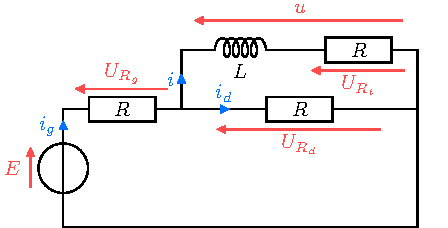
\includegraphics[width=\linewidth]{transRL_q7}
				\captionof{figure}{Schéma à $t=t_1^{+}$.}
			\end{center}
		\end{minipage}
		\vspace{20pt}
		\nitem{8} \label{Q:perm2}\noindent
		\begin{minipage}[t]{.49\linewidth}
			En régime permanent, la bobine se comporte comme un fil. Le
			circuit se résume à un générateur alimentant trois résistances.
			On associe les deux résistances en parallèle et on applique la
			formule du pont diviseur de tension~:
			\[
				u(t_2^-)=\frac{R/2}{R+R/2}E
				\Ra
				\boxed{u(t_2^-)=\frac{E}{3}}
				\Ra
				\boxed{i(t_2^-)=\frac{E}{3R}}
			\]
		\end{minipage}
		\hfill
		\begin{minipage}[t]{.49\linewidth}
			~
			\vspace{-40pt}
			\begin{center}
				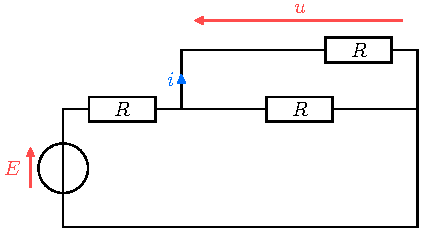
\includegraphics[width=\linewidth]{transRL_q8}
				\captionof{figure}{Schéma à $t=t_2^{-}$.}
			\end{center}
		\end{minipage}
		\nitem{3} On utilise le circuit en régime transitoire pour $t\in]t_1,t_2[$.
		\begin{DispWithArrows*}[]
			E &= R(i_g) + u
			\Arrow{$i_g = i+i_d$}
			\\\Lra
			E &= Ri + Ri_d + u
			\Arrow{$Ri_d = u$}
			\\\Lra
			E &= Ri + 2u
			\Arrow{$u = L \dv{i}{t} + Ri$}
			\\\Lra
			E &= Ri + 2 L\dv{i}{t} + 2Ri
			\Arrow{Forme canonique}
			\\\Lra
			\dv{i}{t}+\frac{3R}{2L}i &= \frac{E}{2L}
			\Arrow{On identifie}
			\\\Ra
			\Aboxed{\tau_2=\frac{2L}{3R} &\qet A_2=\frac{E}{2L}}
		\end{DispWithArrows*}
		\nitem{6} La solution est la somme de la solution de l'équation homogène et
		d'une solution particulière~:
		\[
			i(t)=i_h(t)+i_p(t)=B_2\exp(-t/\tau_2)+\frac{E}{3R}
		\]
		On utilise la condition initiale pour déterminer la constante $B_2$~:
		\[
			i(t_1)=\frac{E}{2R}=B_2e^{-t_1/\tau_2}+\frac{E}{3R}
			\qso B_2=\frac{E}{6R}e^{t_1/\tau_2}
		\]
		\[
			\boxed{
			i(t)= \frac{E}{6R}\left (2+e^{-(t-t_1)/\tau_2}  \right )
			\quad\mbox{pour } t\in]t_1;t_2[
			}
		\]
		Quand on atteint le régime permanent,
		$\lim_{(t-t_1)\gg \tau_2}i(t)= E/(3R)$, ce qui cohérent avec la
		réponse à la question~\ref{Q:perm2}.
		\mitem{4} \[
			\boxed{
			u(t) = L\dv{i}{t} + Ri =
			\frac{E}{6}\left [2-\frac{1}{2}e^{-(t-t_1)/\tau_2}  \right ]
			}
		\]
		On vérifie que $u(t_1)=E/4$.

		Quand on atteint le régime permanent,
		$\lim_{(t-t_1)\gg \tau_2}u(t)= E/3$, ce qui cohérent avec la réponse
		à la question~\ref{Q:perm2}.
	\end{enumerate}
}
\subsection{Étude pour $t\in]t_2;+\infty[$}
\switch{
	\begin{enumerate}
		\item En supposant que le régime permanent est atteint à l'instant
		      $t_2^-$,  exprimer $i(t_2^+)$ et $u(t_2^+)$.
		\item Exprimer $i$ et $u$ pour $t\rightarrow +\infty$.
		\item Établir l'équation différentielle vérifiée par $i(t)$ pour
		      $t\in]t_2,+\infty[$. Montrer qu'elle peut se mettre sous la forme~:
		      \[
			      \dv{i}{t}+\frac{1}{\tau_3}i=A_3
		      \]
		      Exprimer les constantes $\tau_3$ et $A_3$ en fonction des données du
		      problème.
		\item Résoudre cette équation différentielle en supposant qu'à l'instant
		      $t=t_2^-$ le circuit est en régime permanent. On exprimera $i$ en
		      fonction de $E$, $R$, $\tau_3$ et $t$ pour $t\in]t_2,+\infty[$.
		\item Exprimer $u(t)$ pour $t\in]t_2,+\infty[$.
	\end{enumerate}
}{
	\begin{enumerate}
		\nitem{3} \noindent
		\begin{minipage}[t]{.49\linewidth}
			La branche contenant le générateur est ouverte donc n'a aucune
			influence sur le circuit et n'est pas représentée.
			Par continuité du courant circulant à travers une bobine~:
			\[
				\boxed{i(t_2^+)=i(t_2^-)=\frac{E}{3R}}
				\Ra
				\boxed{u(t_2^+)=-\frac{E}{3}}
			\]
		\end{minipage}
		\hfill
		\begin{minipage}[t]{.49\linewidth}
			~
			\vspace{-40pt}
			\begin{center}
				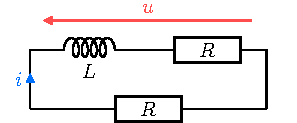
\includegraphics[width=\linewidth]{transRL_q12}
				\captionof{figure}{Schéma à $t=t_2^{+}$.}
			\end{center}
		\end{minipage}
		\nitem{2} En régime permanent, la bobine se comporte comme un fil. Le circuit
		se résume à deux résistances sans alimentation~:
		\[
			\boxed{i(+\infty)=0\qet u(+\infty)=0}
		\]
		\nitem{2} On utilise le circuit en régime transitoire pour $t\in]t_2,+\infty[$.
		On applique la loi des mailles
		\begin{gather*}
			L\dv{i}{t}+2Ri=0\qso \dv{i}{t}+\frac{2R}{L}i=0
			\\\Ra
			\boxed{\tau_3=\frac{L}{2R}\qet A_3=0}
		\end{gather*}
		\mitem{2}
		\begin{DispWithArrows*}[groups]
			i(t) &= B_3\exr^{-t/\tau_3}
			\Arrow{Condition initiale}
			\\
			\text{or,} \quad
			i(t_2) &= B_3\exr^{-t_2/\tau_3} = \frac{E}{3R}
			\Arrow{On isole $B_3$}
			\\\Lra
			\Aboxed{B_3 &= \frac{E}{3R}\exr^{t_2/\tau_3}}
			\Arrow[new-group]{On combine}
			\\\Ra
			\Aboxed{
			i(t) &= \frac{E}{3R}e^{-(t-t_2)/\tau_3}
			\quad \text{pour} \quad
			t\in]t_2;+\infty[
			}
		\end{DispWithArrows*}
		\nitem{2} Par la loi d'Ohm :
		\[
			\boxed{
			u(t) = -Ri =
			-\frac{E}{3}e^{-(t-t_2)/\tau_3}
			\quad\mbox{pour } t\in]t_2;+\infty[
			}
		\]
	\end{enumerate}
}
\subsection{Combinaison des régimes}
\switch{
	\begin{enumerate}
		\item Tracer l'allure de $i$ en fonction du temps, pour $t\in]0;+\infty[$
		      sur la Figure~\ref{fig:annexe_p2-2} en annexe. On fera apparaître les
		      constantes de temps $\tau_1$, $\tau_2$ et $\tau_3$ sur ce graphique,
		      ainsi que les valeurs de $i$ à chaque changement de régime.
		\item Tracer l'allure de $u$ en fonction du temps, pour $t\in]0;+\infty[$
		      sur la Figure~\ref{fig:annexe_p2-3} en annexe. On fera apparaître les
		      constantes de temps $\tau_1$, $\tau_2$ et $\tau_3$ sur ce graphique,
		      ainsi que les valeurs de $u$ à chaque changement de régime.
	\end{enumerate}
}{
	\begin{enumerate}
		\nitem{7} On calcule les temps~:
		\[
			\tau_3=\tau_1=\SI{0,5}{\milli\second}
			\qet
			\tau_2=4\tau_1/3=\SI{0,66}{\milli\second}
		\]
		Voir Figure~\ref{fig:annexe_p2-2_corr}
		\nitem{5} Voir Figure~\ref{fig:annexe_p2-3_corr}
	\end{enumerate}
}

\switch{
	\newpage
	\chapter*{Annexe~: exercice 2}
	\begin{tikzpicture}[remember picture, overlay]
		\node[anchor=north west, align=left]
		at ([shift={(1.5cm,0)}]current page.north west)
		{\\[5pt]\Large\bfseries Nom~:\\[10pt]\Large\bfseries Prénom~:};
		\node[anchor=south east, align=right]
		at ([shift={(-1.5cm,1.5cm)}]current page.south east)
		{\Large\bfseries Copie\hspace{.5cm}/\hspace{.5cm}};
	\end{tikzpicture}

	\vfill
	\begin{figure}[htbp!]
		\centering
		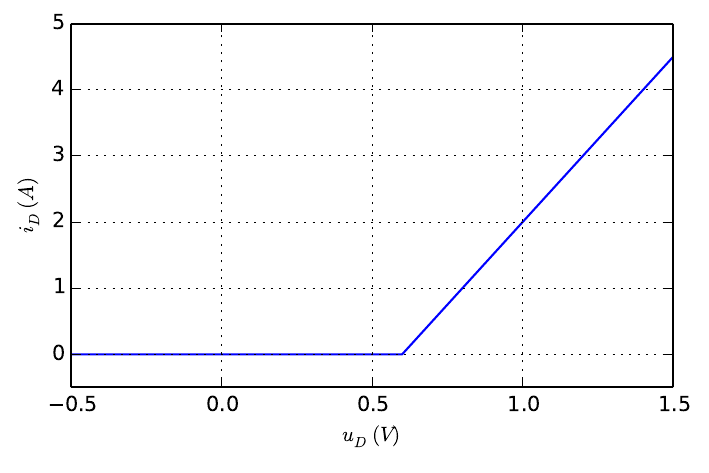
\includegraphics[width=\linewidth]{diode_annexe}
		\caption{Annexe question 8.}
		\label{fig:diode_annexe}
	\end{figure}
	\vfill

	\chapter*{Annexe~: problème 2}

	\begin{figure}[htbp!]
		\centering
		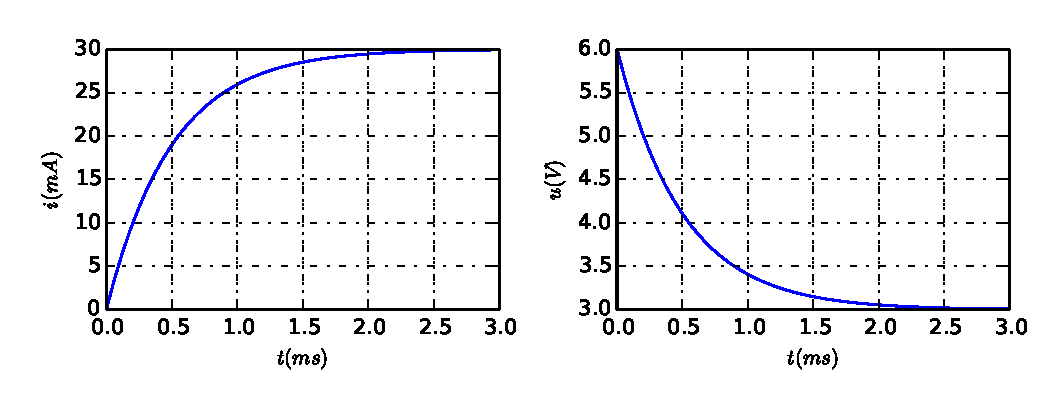
\includegraphics[width=\linewidth]{transRL_trace.pdf}
		\vspace{-40pt}
		\caption{Annexe question 6.}
		\label{fig:annexe_p2-1}
	\end{figure}
	\begin{figure}[htbp!]
		\centering
		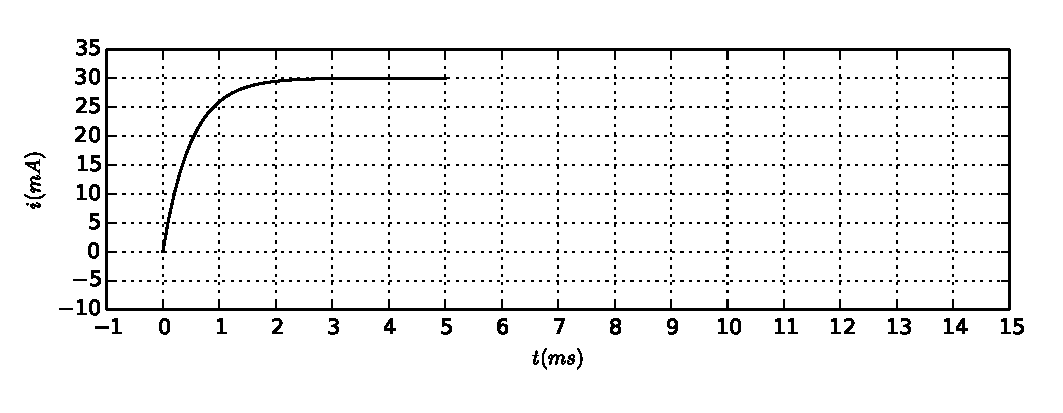
\includegraphics[width=\linewidth]{transRL_tracei.pdf}
		\vspace{-40pt}
		\caption{Annexe question 17.}
		\label{fig:annexe_p2-2}
	\end{figure}
	\begin{figure}[htbp!]
		\centering
		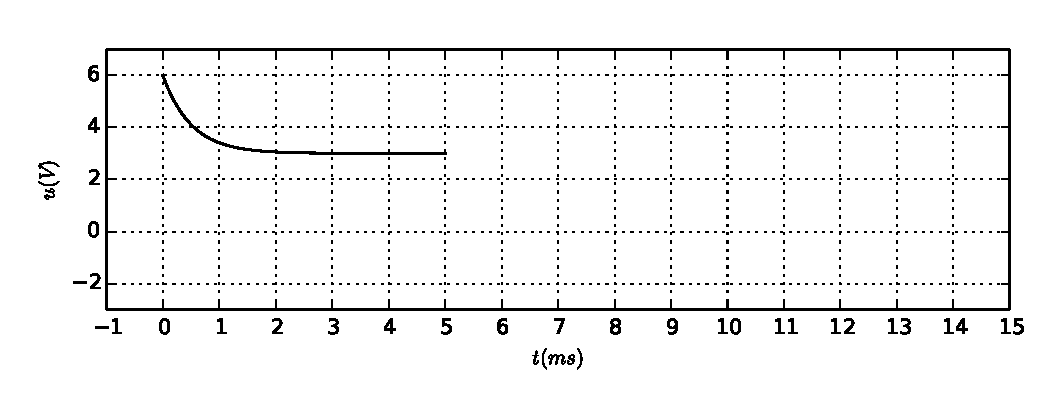
\includegraphics[width=\linewidth]{transRL_traceu.pdf}
		\vspace{-40pt}
		\caption{Annexe question 18.}
		\label{fig:annexe_p2-3}
	\end{figure}

}{
	\newpage
	\chapter*{Annexe~: exercice 2}
	\vfill
	\begin{figure}[htbp]
		\centering
		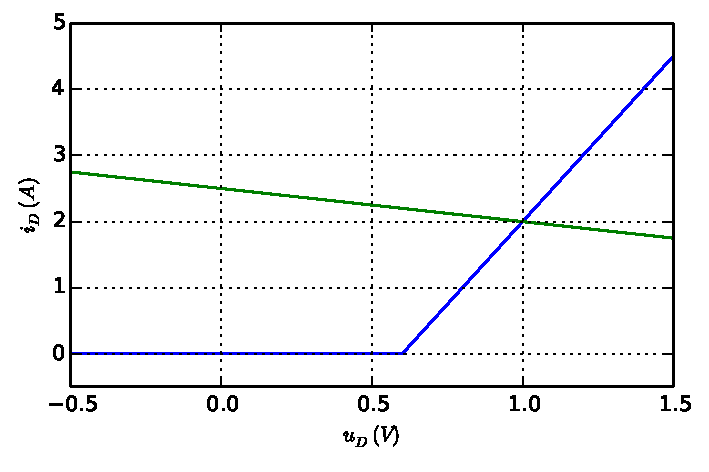
\includegraphics[width=\linewidth]{diode_annexecorr}
		\caption{Annexe question 8.}
		\label{fig:diode_annexecorr}
	\end{figure}
	\vfill

	\chapter{Annexe~: problème 2}
	\begin{center}
		\subimport{figures/P2/}{transRL_tracecorr.pdf_tex}
		\captionof{figure}{Annexe question 6.}
		\label{fig:annexe_p2-1_corr}
	\end{center}
	\begin{center}
		\subimport{figures/P2/}{transRL_traceicorr.pdf_tex}
		\captionof{figure}{Annexe question 16.}
		\label{fig:annexe_p2-2_corr}
	\end{center}
	\begin{center}
		\subimport{figures/P2/}{transRL_traceucorr.pdf_tex}
		\captionof{figure}{Annexe question 17.}
		\label{fig:annexe_p2-3_corr}
	\end{center}
}
\vspace{-20pt}
\end{document}
